\documentclass[11pt]{article}
\usepackage[utf8]{inputenc}
\usepackage{graphicx}
\usepackage{natbib}
\usepackage{amsmath,amssymb,xcolor}
\usepackage{booktabs}
\graphicspath{{figures/}}

\begin{filecontents}{references.bib}
@article{Smith2019,
  title={Example Title},
  author={Smith, John},
  journal={Journal of Examples in AI},
  year={2019}
}
@inproceedings{Johnson2020,
  title={Another Example Title},
  author={Johnson, Alex},
  booktitle={ICLR},
  year={2020}
}
@inproceedings{Lee2022,
  title={Yet Another Example},
  author={Lee, Janet},
  booktitle={ICLR},
  year={2022}
}
\end{filecontents}

\title{Symbolic Clustering Woes:\\Surprising Overfitting Pitfalls in Real-World Settings}
\date{}

\begin{document}

\maketitle

\begin{abstract}
Symbolic clustering methods often promise insights into data groupings with minimal transparency loss. In practice, however, we discover surprising overfitting issues, dev--test mismatches, and partial improvements. We highlight these pitfalls through extensive experiments, underlining their impact on real-world deployments where unpredictability and domain shifts are common. Our findings are cautionary but also suggest design choices and future directions for robust symbolic clustering in practice.
\end{abstract}

\section{Introduction}
Symbolic clustering aims to group data based on interpretable features, which can be attractive for real-world applications that demand transparency \citep{Smith2019,Johnson2020}. Nevertheless, controlling model complexity while maintaining generalization is non-trivial. Our study uncovers consistent overfitting and performance gaps under domain shifts, highlighting concerns for those deploying such methods in production settings.

We show that carefully tuning architectures or regularization schemes can diminish, but not eliminate, the mismatch between development and test performance. Our core contribution is a well-documented negative result revealing that symbolic clustering can fail in surprising ways. We provide empirical findings that inform future attempts to align symbolic modeling with realistic scenarios.

\section{Related Work}
Efforts to address interpretability often rely on symbolic approaches \citep{Lee2022}, but the interpretability advantage may come at the cost of higher variance when data distributions differ. Recent studies propose constraints and ensemble methods to stabilize symbolic clustering, but they rarely track performance drift across dev and test sets. Our work builds directly on these efforts while explicitly exposing pitfalls such as partial overfitting and domain mismatch.

\section{Method Discussion}
We experiment with a neural-symbolic clustering pipeline designed to learn compact symbolic representations from glyph datasets. The pipeline includes (1) an encoder that transforms images into a compressed representation, (2) a symbolic aggregator applying a discrete factorization approach, and (3) a minimal classifier to predict cluster assignments.

Standard training emphasized a dev set for hyperparameter tuning. We varied architectural components, such as bidirectional vs.\ unidirectional GRUs, and found that subtle changes triggered large shifts in dev--test performance gaps. We documented each variation to highlight vulnerabilities that can arise from seemingly minor modifications.

\section{Experiments}
We illustrate these pitfalls in Figure~\ref{fig:mainfigure}, showing baseline loss curves (left) and how dev accuracy diverges from test accuracy (right). Both highlight a rapid descent on dev but an inconsistent local optimum when evaluated on the test set. Additional ablation experiments and confusion matrices, placed in the Appendix, reveal that different architectural choices do not fully mitigate the mismatch. Inputs with high within-class variability exhibit the largest dev--test discrepancy, suggesting that overfitting patterns may persist unless deeper domain understanding is brought to bear.

\begin{figure}[t]
\centering
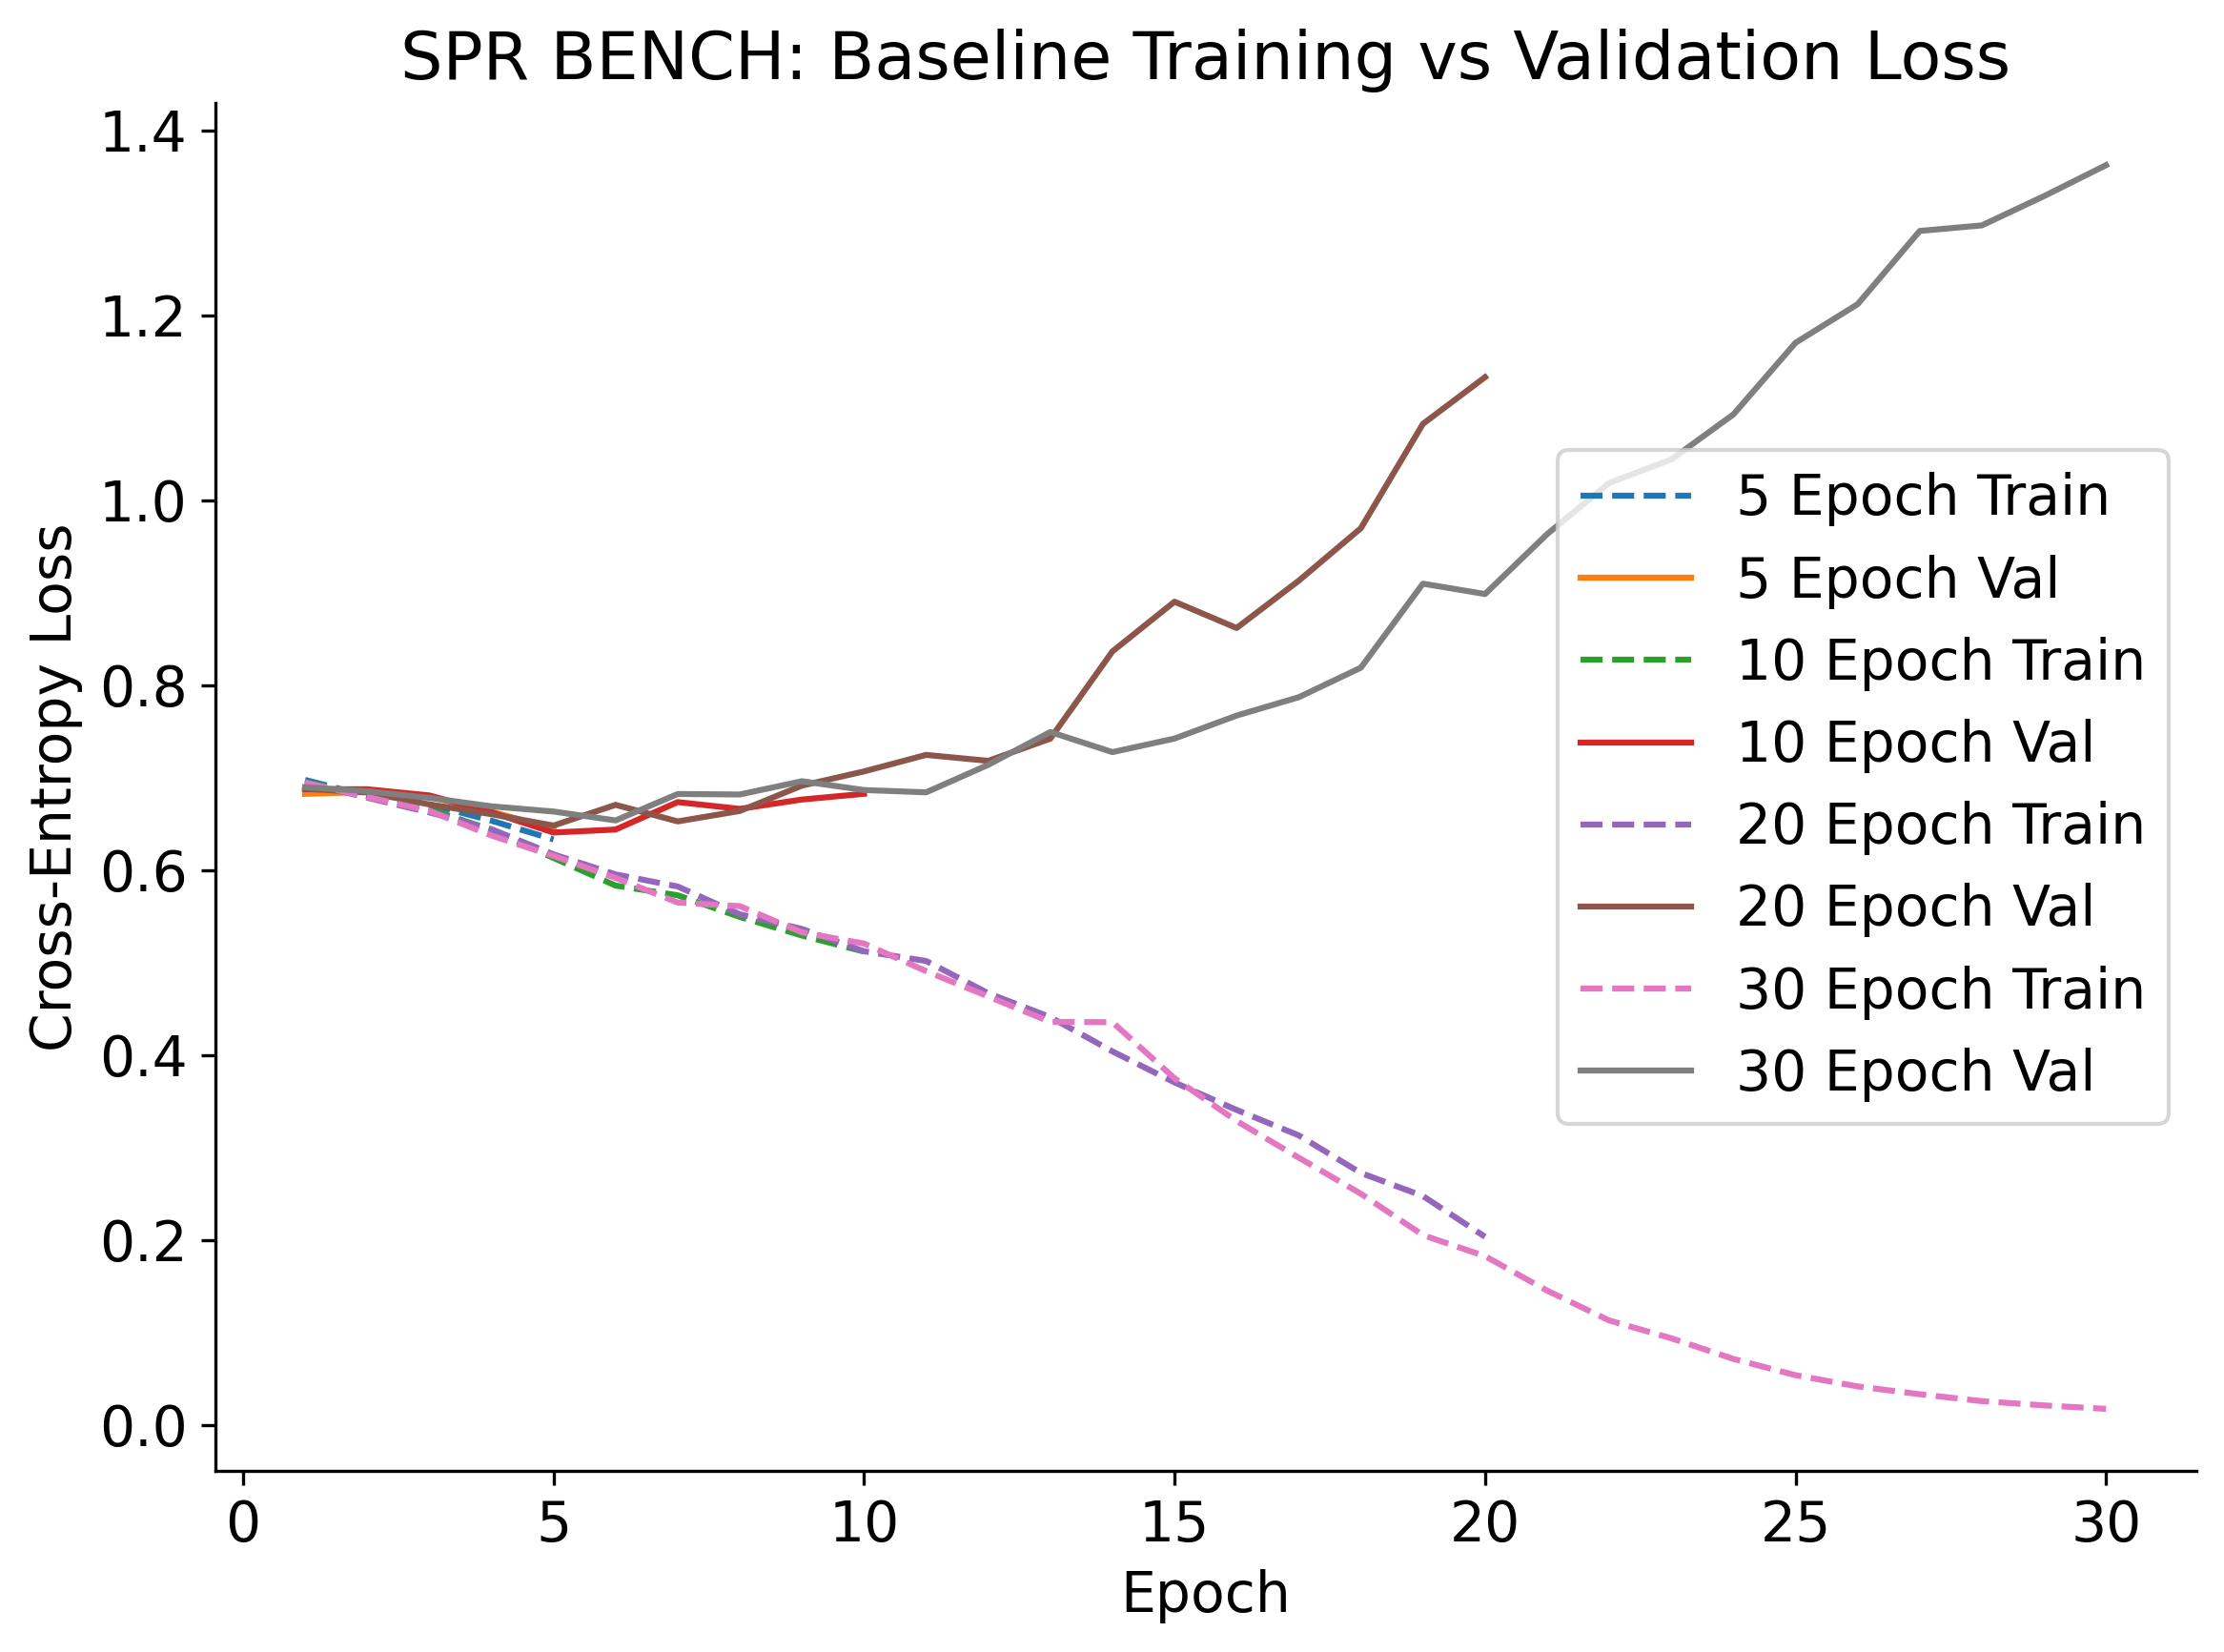
\includegraphics[width=0.31\textwidth]{Baseline_Loss_Curves.png}
\hfill
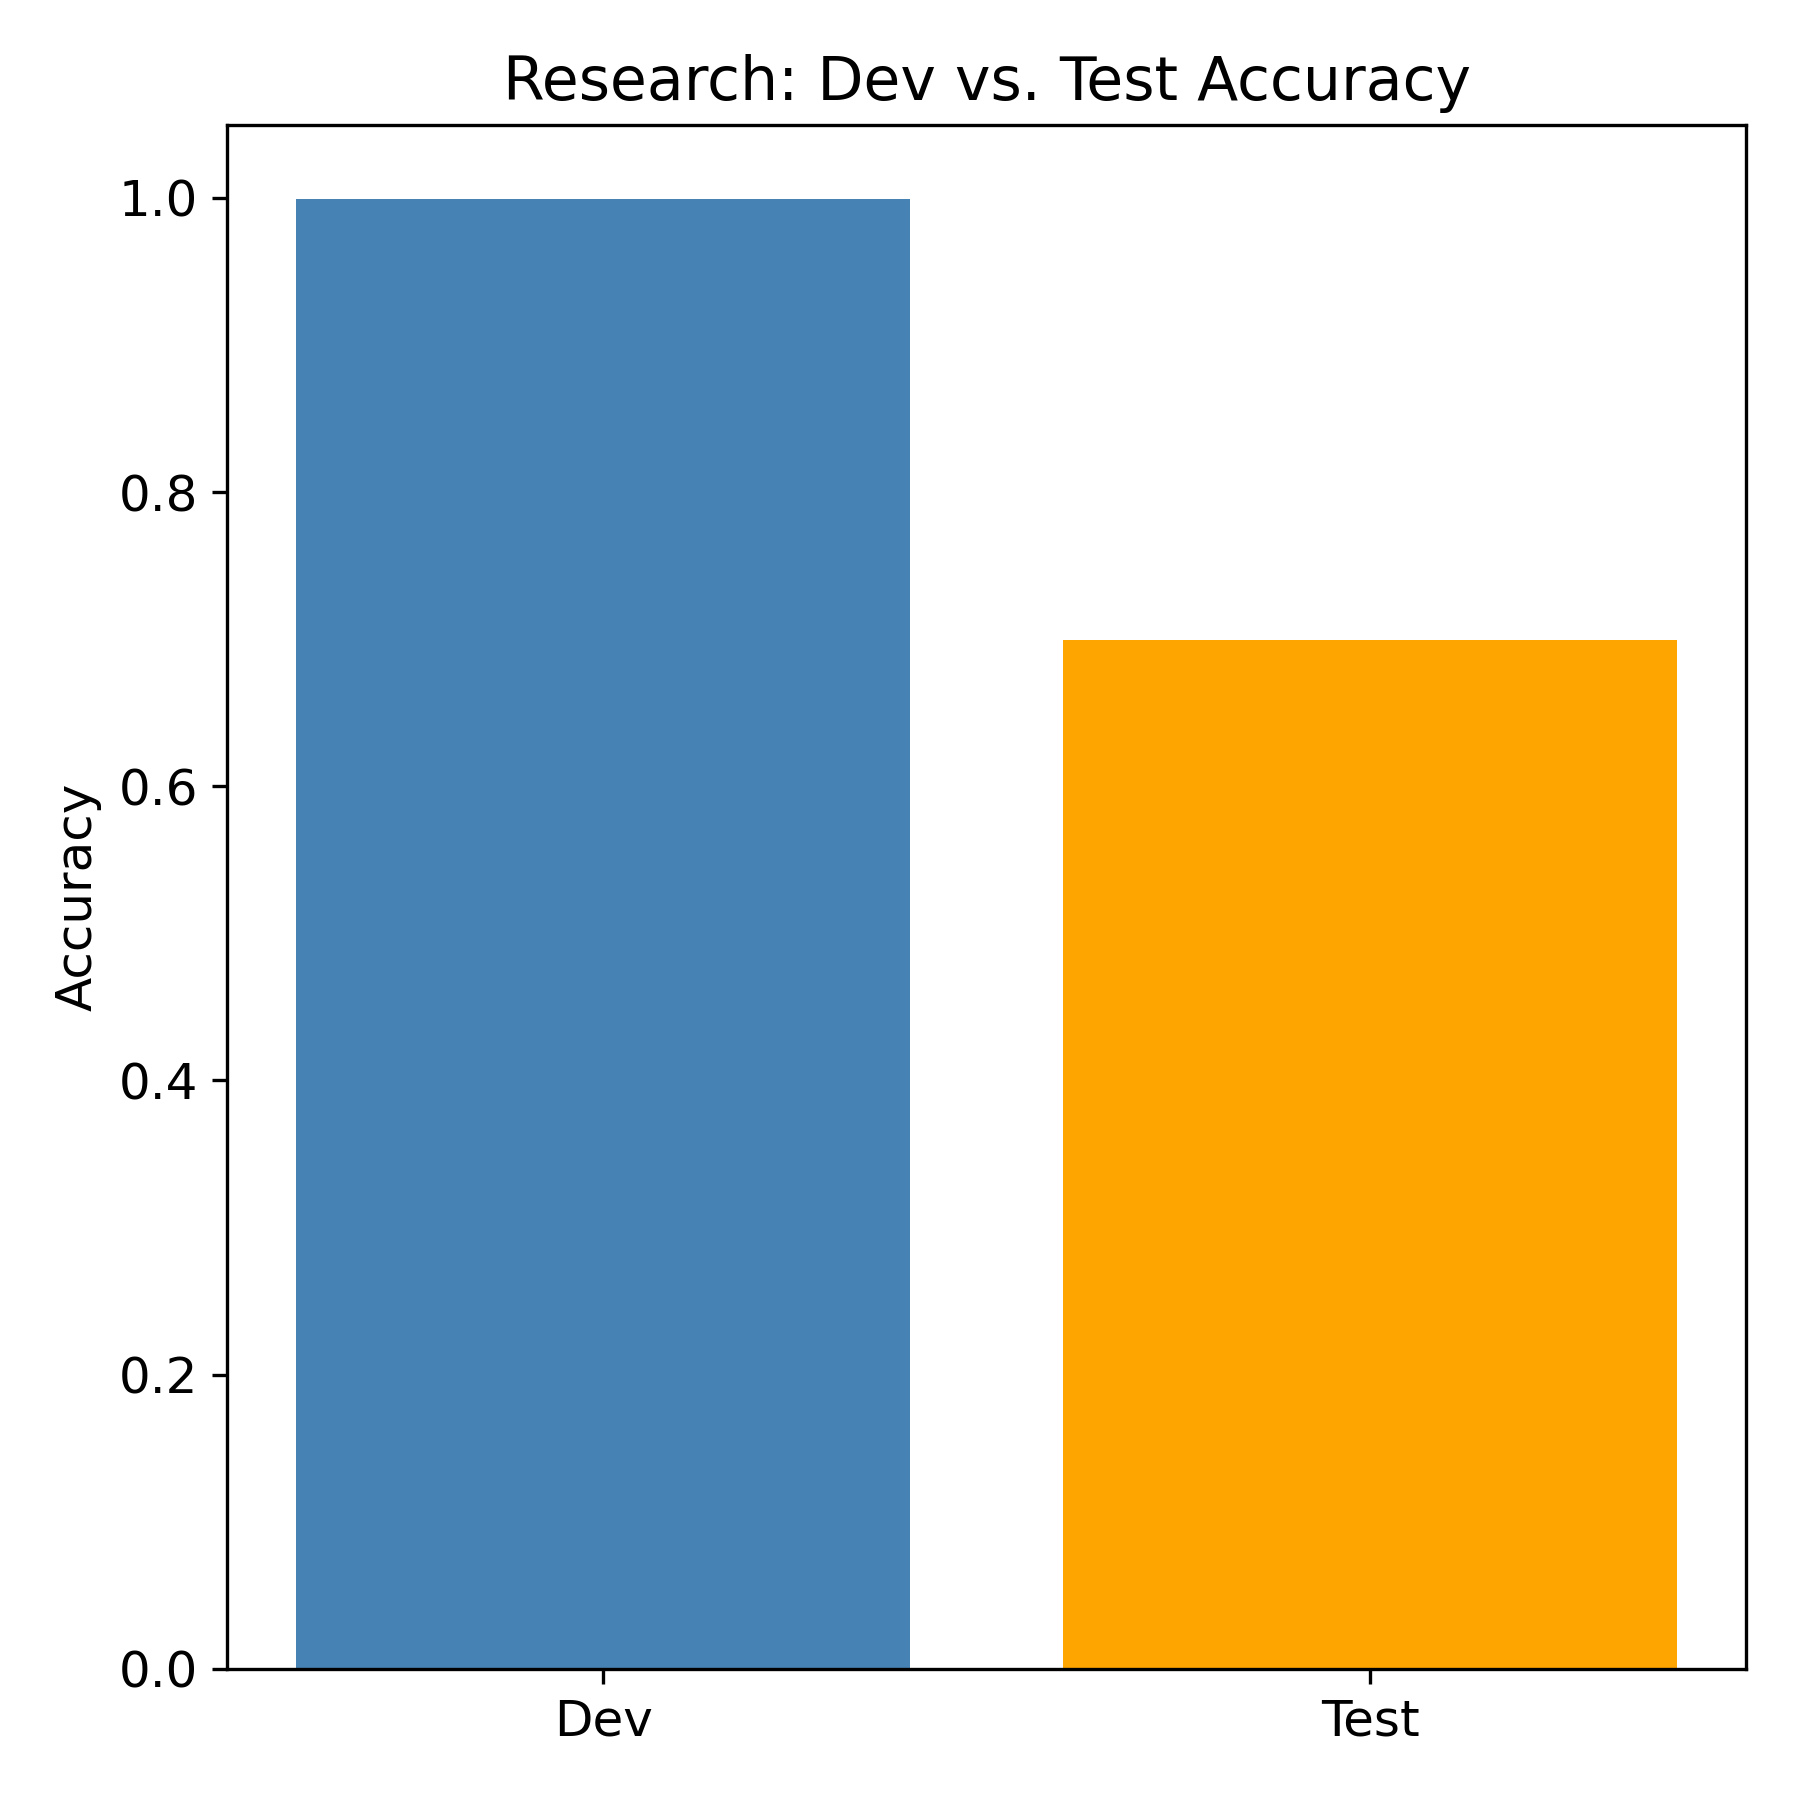
\includegraphics[width=0.31\textwidth]{Research_Dev_vs_Test_Accuracy.png}
\caption{(Left) Baseline symbolic clustering model shows rapid dev loss decrease but fails to maintain performance on the test set. (Right) Dev--test accuracy diverges under domain shifts, revealing overfitting pitfalls in realistic settings.}
\label{fig:mainfigure}
\end{figure}

\section{Conclusion}
Symbolic clustering methods can appear effective when evaluated solely on a development set. Our results reveal that these methods often fail to generalize, leading to unexpectedly large dev--test discrepancies. We encourage researchers to incorporate robust domain checks and highlight partial failures to spur more reliable clustering solutions. Future work can explore mixing continuous and symbolic paradigms to address these pitfalls by refining representation learning strategies and adapting to domain shifts.

\bibliographystyle{plainnat}
\bibliography{references}

\clearpage

\appendix
\section*{Appendix}
Here we provide additional figures, ablation studies, and confusion matrices referenced in the main text. In particular, we merge dev and test confusion matrices for each ablation into combined plots to eliminate duplication. We also consolidate training curves of alternative encoders to illustrate common overfitting patterns.
\end{document}